%
%  $Author: awl8049 $
%  $Date: 2008/01/08 22:09:49 $
%  $Revision: 1.18 $
%
\documentclass[times, 10pt,twocolumn]{article} 
\usepackage{latex8}
\usepackage{times}
\usepackage{graphicx}
\usepackage{authblk}
\usepackage{amsmath}
\usepackage{pdfsync}
\pagestyle{empty}
\begin{document}
\title{VMpower: Virtualization for Energy Conservation in Clusters With
  Heterogeneous Nodes}
\author[*]{Adam Lewis}
\author[*]{Soumik Ghosh}
\author[*]{Nian--Feng Tzeng}
\affil[*]{Center for Advanced Computer Studies\\ 
University of Louisiana at Lafayette\\
Lafayette, LA 70504, USA\\ 
\{awlewis,sxp1667,tzeng\}@cacs.louisiana.edu
}
\maketitle
\thispagestyle{empty}
\begin{abstract}
Application servers have characteristics that make energy conversation
difficult.  Virtualization is a tool that can be used to simplify the process
of energy conservation in server clusters.   In this work, we introduce a
framework that combines virtualization, load balancing, and power management
to reduce the energy consumption of a cluster of application servers.   We
evaluate the framework using experiments based on statistical principles to
measure the improvement that our framework provides over other proposed schemes.
\end{abstract}
\section{Introduction}
\label{introduction}
Large data centers host hundreds and thousands of servers that require complex
and costly cooling solutions.  Providing proper cooling has become more
difficult as servers are grouped into server clusters with greater numbers of
more powerful and densely populated nodes result in greater energy consumption
across the entire cluster.

Application servers have characteristics that make energy conservation
particularly difficult \cite{Bianchini2004}.  Typical workloads on such
servers lead to intensive CPU and memory use which means energy conservation
mechanisms must not cause excessive overhead under moderate and heavy loads.
In addition, such workloads tend to require applications maintain some form of
soft state that is typically not replicated across nodes in a server
cluster. As result, mechanisms that look to shut down portions of a cluster
would require applications to consider migration of that state across nodes.

A possible approach for managing this situation is \textit{virtualization}.
In a virtualized environment applications run on a virtual server and one or
more virtual servers are mapped onto physical servers in the cluster.  A
virtualized environment provides many advantages within the data center such
as application isolation, server consolidation, and better utilization of
resources across the data center.

A great advantage of virtualization is the ability to remap physical resources
to virtual servers in order to better handle workload dynamics.  Additional
resources can be added to the virtual server if idle resources are available
on the physical server or the virtual server can be migrated to a less loaded
physical server.  Recent research \cite{Grit2006} \cite{Wood2007}
\cite{Govindan2007} has considered using virtual server migration to reduce
the complexity of load balancing for better performance.  In this work, we
consider the use of virtual machine migration for energy conservation and
thermal management.

The remainder of this paper is organized into five sections.  Section
\ref{sec:power} describes the power model that is the basis of our
framework. The method used to implement the power model in an
implementation framework is described in section \ref{sec:Method} In
section \ref{sec:system} we describe the architecture of the VMpower
framework and the infrastructure that supports that architecture.  We
provide an experimental analysis of the behavior of the framework in
\ref{sec:experiment}. A review of related work is provided in Section
\ref{sec:related}.  Finally, we review the conclusions drawn from this
work and discuss future work in Section \ref{sec:future}.

\section{Power Model}
\label{sec:power}
The development of an accurate predictor that determines where state must be
migrated requires that we have an effective model of the power consumption and
thermal loads of a cluster. 
 
Servers are rated by their manufacturer with a maximum power draw that is used
to estimate the power and cooling infrastructure required to safely install
this machine in the data center.   Typically, these ratings are conservative
in nature and are typically calculated by adding up the worst case power
consumption of the components in the server.  In Fan, \textit{et. al.}
\cite{Fan2007}, it was found that a more accurate measurement of power
consumption is \textit{actual peak power}.

\subsection{Physical Power Model}
\label{sec:powerphysical}
We can express our peak power model in terms of an optimization problem: find
the ideal distribution of requests from clients to servers and amongst servers
such that the demand for resources is not higher than available supply and we
minimize the overall energy consumed by the cluster. \cite{Heath2005}

Our model uses an approach similar to Mantis \cite{Economou2006} where we define
four types of resources in each node and the metrics used to measure the
resource: 
\begin{itemize}
\item $\mu_{CPU}$: CPU utilization
\item $\mu_{memory}$: Off-chip memory access count
\item $\mu_{disk}$: Hard disk I/O rate
\item $\mu_{net}$: Network I/O rate
\end{itemize}
The power consumed by the server is modeled as a linear function of these
metrics over time:
\begin{equation*}
  P_{server}= I + A*\mu_{CPU} + B*\mu_{memory}+C*\mu_{disk}+D*\mu_{net}
\end{equation*}
where $I$ is a constant indicator of power consumption when the system is
idle.  The constants $A$,$B$,$C$, and $D$ are estimated using linear
regression techniques against data traces of common benchmarks.

\begin{table*}
  \centering
  \begin{tabular}{|l|l|l|}
    \hline
    \textbf{Type}&\textbf{Measure}&\textbf{Formula}\\
    \hline
    Server Power Load&Power consumed (watts)&Sum of individual loads\\
    \hline
    UPS w/ Battery&UPS Power System Rating (watts)&$(0.04*Power System Rating)
    +(0.05*Server Power Load)$\\
    \hline
    Power Distribution Unit&PDU Power System Rating (watts)&$(0.01*Power
    System Rating)+(0.02*Server Power Load)$\\
    \hline
  \end{tabular}
  \caption{Server Rack Power Consumption}
  \label{tab:rackpower}
\end{table*}
Servers in data centers are typically mounted in racks of up to forty-eight
servers. The total power load of a server rack is the sum of the servers in
the rack plus the power consumption of the supporting equipment. The UPS,
Power Distribution Unit and other supporting hardware require a certain amount
of power to perform their function \cite{APC2003}.  Table \ref{tab:rackpower}
shows how we extend our model for a single server across the an entire server
rack.  We sum the power consumed per each rack if the cluster is built from
multiple server racks.

\subsection{Effect of Virtual Machines on Physical Power Model}
\label{sec:powervirtual}
How do virtual machines impact this approach?  Our power model is estimating
the power consumption of the physical machine.  At the physical machine layer,
the hypervisor is responsible for translation of the virtual I/O requests to
physical requests in the operating systems.  This introduces additional
overhead onto CPU to translate the request. 

We can model the power consumed by each virtual machine in the same manner
that we model the power consumed by the physical machine where the total
power consumed by the physical machine is represented by 
\begin{equation*}
  P_{node}=P_{D_{0}}+\sum_{i=1}^{num\_nodes}P_{VM_{i}}
\end{equation*}
\begin{equation*}
  P_{VM}= i + a*\phi_{CPU} + b*\phi_{memory}+c*\phi_{disk}+d*\phi_{net}
\end{equation*}
where
\begin{itemize}
\item $\phi_{CPU}$: CPU utilization
\item $\phi_{memory}$: Off-chip memory access count
\item $\phi_{disk}$: Hard disk I/O rate
\item $\phi_{net}$: Network I/O rate
\end{itemize}
If we rewrite the values of $\phi$ in physical model terms, we need to add
additional terms to the CPU utiliziation to account for the translation
overhead within the hypervisor:
\begin{eqnarray*}
\lefteqn{P_{VM} = i + a*\phi_{CPU}+}\\
& &b*(w_{memory}+t_{memory})+\\
& &c*(w_{disk}+t_{disk})+\\
& &d*(w_{net}+t_{net})
\end{eqnarray*}

where the qunatities $t_{memory}$, $t_{disk}$, and $t_{net}$ are the
additional CPU workload required to translate the virtual machine device
access into to the physical request.

We can rewrite this equation as follows:
\begin{eqnarray*}
\lefteqn{P_{VM}= i + a*\phi_{CPU}+}\\
& &b_{1}*\phi_{memory}+b_{2}*t_{memory})+\\
& &c_{1}*\phi_{disk}+c_{2}*t_{disk}+\\
& &d_{1}*\phi_{net}+d_{2}*t_{net}
\end{eqnarray*}

By doing so, we can use the same linear regression techniques to
estimate the values of the constants in the equation.

\subsection{Optimization of Cluster Energy Consumption}
\label{sec:optimize}
We can now frame the energy conservation problem as an optimization
problem: minimize the power consumed by the cluster in order to address a given
CPU, disk, memory, and network workload given the constraint that the
execution of the workload not violate a pre-determined service
level. We define the serivice-level agreement (SLA) as requiring the
incoming server requests to not execeed a targeted average response time.

Given this, we can phrase the optimiziation problem in terms of an
objective functions based on the power model from the previous sections
and a set of constraints.  We seek some partition of the cluster
$(m1,m2,\dotsb,m_{n})$ such that the objective function 
\begin{equation*}
  \begin{pmatrix}
    P^{node_{1}}\\
    P^{node_{2}}\\
    P_{D_{0}}^{node_{3}}\\
    P_{VM_{1}}^{node_{3}}\\
    P_{VM_{2}}^{node_{3}}\\
    \dotsb
  \end{pmatrix} =
  \begin{pmatrix}
    \mu_{CPU}^{node_{1}}\\
    \mu_{CPU}^{node_{2}}\\
    \mu_{CPU_{D_{0}}}^{node_{3}}\\
    \mu_{CPU_{VM_{1}}}^{node_{3}}\\
    \mu_{CPU_{VM_{2}}}^{node_{3}}\\
    \dotsb
  \end{pmatrix} +
  \begin{pmatrix}
    \mu_{Memory}^{node_{1}}\\
    \mu_{Memory}^{node_{2}}\\
    \mu_{Memory_{D_{0}}}^{node_{3}}\\
    \mu_{Memory_{VM_{1}}}^{node_{3}}\\
    \mu_{Memory_{VM_{2}}}^{node_{3}}\\
    \dotsb
  \end{pmatrix} +
\dotsb
\end{equation*}
is minimized under the following contstraints
\begin{itemize}
\item the system does not violate the service level agreement such that
  the average response time $t_{w}$ for the workload does not exceed
  some maximum limit $t_{max}$.
\item the number of nodes $i$ selected is less than or equal to $n$, the
  number of nodes in the cluster.
\end{itemize}

\section{Method}
\label{sec:powerapply}
So, given our power model, how can we reduce the overall power consumption?
Prior work \cite{Pinheiro2003} \cite{Hermenier2007} has taken the approach of
complete shutdown of the unused nodes in the cluster in a technique described
as ``Vary On, Vary Off'' or ``VOVO''.  This technique significantly
reduces the overall power consumption but it has a negative impact on Quality
of Service (QoS) given the time required to bring cluster nodes back
on-line. Rather than turning off the unused physical nodes, we propose either
suspending or shutting down unused virtual machines in the cluster but not
turning off the physical host.  This avoids
the issues with physical shutdown of the machine while still reducing the
values of $\mu_{CPU}$, $\mu_{memory}$, $\mu_{disk}$, and $\mu_{net}$ in
our model. Our method has two distinct phases: calibration and
prediction. 

\subsection{Calibration}
\label{sec:methodcalibrate}
The calibration phase is neccessary because the values of the constants
in our power model are different depending upon hardware and network
configuration. A series of benchmark workloads are executed on the
target configuration to determine the energy consumed and values for
CPU, disk, memory, and network workloads.   Linear regression techniques
are used to estimate the values of the constants in our model.

\subsection{Prediction}
\label{methodprediction}
Our model is the foundation for a power predictor framework that
dynamically solves the optimization problem in the previous section. At
each time step $t$, the predictor will produce a partition of the
cluster in use at time step.  Nodes not in the partition will be
disabled.  Physical nodes will be turned off per the ``VOVO''
philosophy.  However, virtual nodes will be either shutdown by the VM
hypervisor or suspended by the VM hypervisor.   We evaluate the energy
consumption impacts of both schemes.

\section{Implementation Framework}
\label{sec:system}
The VMPower framework must address two key requirements:
\begin{itemize}
\item The framework must be able to operate with any application server.
\item The framework must be transparent to the application server and require
  no changes in the application server.
\end{itemize}
\begin{figure}[h]
 	\centering
	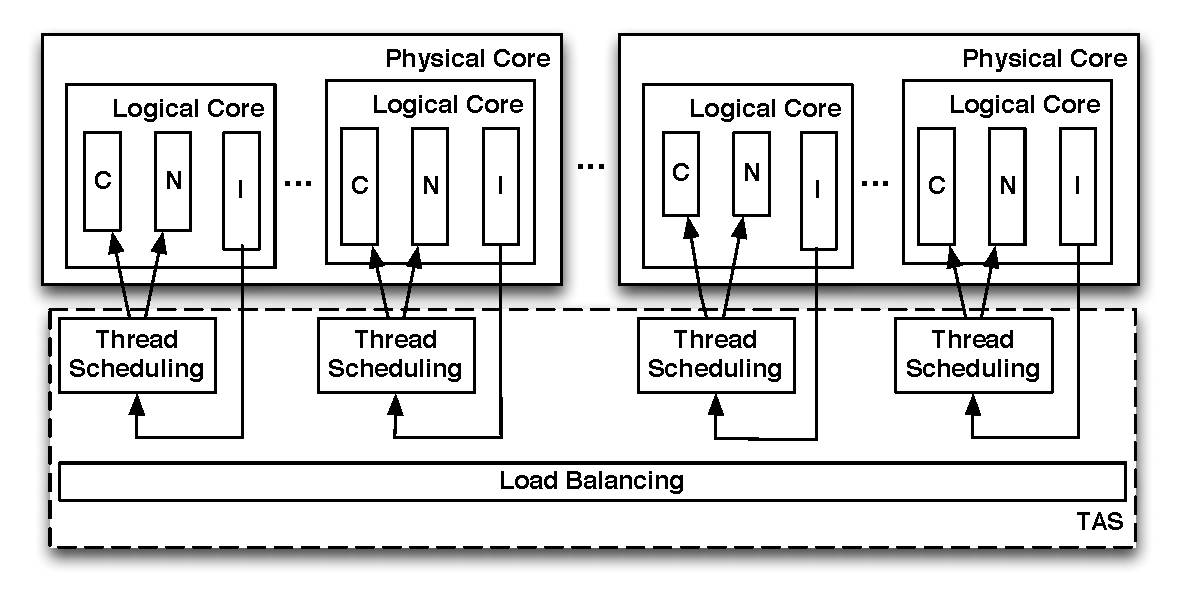
\includegraphics[width=\linewidth]{architecture.pdf}
   	\caption{System Architecture}
  	\label{architecture}
\end{figure}
Figure \ref{architecture} shows the architecture of the framework where we
a cluster of servers composed of a \textit{head node} and one or more
\textit{compute nodes}.  The head node manages the cluster through three key
services:
\begin{itemize}
\item \textit{migration}: a service that initiates and manages the migration of
  virtual servers to different physical nodes in the cluster
\item \textit{load balancing}: a service that is responsible for distributing
  incoming application requests to the virtual servers in the cluster.
\item \textit{cluster health monitoring}: a service that monitors key
  performance characteristics of the physical compute nodes plus utilization
  of the virtual servers on the compute node.
\end{itemize}
Each of the compute nodes runs the minimum set of software required to operate
the virtualization hypervisor.  The virtualization hypervisor manages one or
more application virtual servers (AVS) where each AVS contains an instance of
the application server software (for example, the Tomcat application server).

The VMpower framework is built using the XEN virtualization middle-ware
\cite{Abels2005}\cite{Barham2003}\cite{Chisnall2007}; however, our
technique can be used with any virtualization middle-ware that supports
live migration of virtual machines.

\subsection{Migration}
\label{sec:migration}
The migration facilities in a virtual machine monitor such as XEN provide
three important services \cite{Clark2005}:
\begin{itemize}
\item VM migration allows the application server to be moved from physical
  node to physical node as a single unit.
\item Both kernel-level and application-level memory states can be transferred
  in a consistent and efficient manner.
\item Migration occurs in a way that is transparent to the user.  Thus, the
  user need not be concerned with ``playing nice'' with the operating system
  while the operator can treat the application server as a single unit.
\end{itemize}

In our case, the live migration features in XEN allow us to transparently move
the application virtual servers to less loaded areas of the cluster.

\subsection{Load balancing}
\label{sec:loadbalance}
Application server clients need to have a single, consistent view of the
application server.  The load balancing service on the head node is
responsible for routing the incoming requests to the AVS in the cluster. The
load balancing service is based on the Linux Virtual Server (LVS)
\cite{LVS2006} \cite{Zha2000}.  LVS is a 4-layer load balance that provides IP
fail-over capabilities.  In our framework, we use the IP Tunneling feature of
LVS so that the head node is responsible for scheduling requests to the
Application Virtual Servers in the cluster.  Each AVS is responsible for
sending replies back to the sender.

\subsection{Cluster health monitoring}
\label{sec:health}
The health monitoring system is based on the Ganglia cluster monitoring
package \cite{Ganglia2003}.  Ganglia provides the infrastructure for
collecting information about the state of the cluster.

The health monitor has two major components: the cluster node data collector
and head node aggreator and action daemon. On each cluster node, the data
collector is a service that runs in the physical node operating system that
collects key metrics about the system.   

The node data collector gathers periodic readings of each of the metrics in
our power model. This information is passed back to the head node aggreator
which collects the data and keeps a history of the predicated and actual power
consumption across the cluster.  The aggreator passes hints to the load
balancing service on where nodes need to be migrated in order to lessen the
overall temperature of the cluster.


\section{Experimental Study}
\label{sec:experiment}
We have performed an experimental study of our energy conservation scheme on a
dedicated cluster to answer the following questions:
\begin{itemize}
\item Is the energy savings achieved by  VMpower equal or within an
  acceptable difference to energy conservation schemes that use VOVO?
\item Does using VMpower provide a measurable improvement in the QoS for
  application servers as compared to schemes that use VOVO?
\end{itemize}

\subsection{Experimental Methodology}
\label{sec:Method}
A set of experiments has been performed to test the hypothesis behind each of
the questions asked at the start of this section.  The experiments have been
designed upon the principles of Statistical Design of Experiments (DoE).
DoE \cite{Montgomery2005} is a methodology to efficiently determine the effects
input factors have upon one or more response metrics.  There are three
principles in DoE: Replication, Randomization, and Blocking.  Replication
ensures that the results were not a fluke and reduces the error.
Randomization ensures that no unintended bias is introduced by uncontrollable
factors.  Blocking organizes the trials so that common factors can be examined
concurrently.

There are two types of input factors, qualitative and quantitative.
Quantitative factors are those that can be given a value like number of
wireless nodes or distance from a gateway.  Qualitative factors are those
which cannot be given a value as in surface terrain or routing protocol.  The
R-Squared value tells us how much of the variability in our data can be
contributed to the input factors.

A factorial design consists several input factors are tested at different
levels to and the response metrics are examined.  Each input factor typically
has two levels, a high and a low.  Other common designs include three level
factors and mixed level factors.  Full factorial design means that all
possible combination of factors are tested.  In a $2^{3}$ experiment, 8 trials
are performed.  In a half factorial design, only 4 trials would be performed.
This is done when there is not enough time or resources available to complete
all of the trials.

Once all of the trials have been completed, Analysis of Variance is performed
to determine the factor effects and regression model.  The factor effects tell
us what main effects (those based on individual factors) and interaction
effects (those based on the interaction between the individual factors) are
important to our regression model.  The regression model will give us a
formula that can be used to estimate the response metric based on the input
factors without running any experiments.  DoE has an advantage of typical
one-factor-at-a-time experiments in that it observes the effect of the
interactions of the input factors.  These factors are often overlooked in
one--factor--at--a--time experiments and could be the most important effect
in the regression model.

\subsection{Experiment Environment}
\label{sec:expdesign}
\begin{table}
  \centering
  \label{tab:hardware}
  \begin{tabular}{|l|l|l|}
    \hline
    \multicolumn{2}{c}{\bf{Dell PowerEdge 1950}}&Sun v20s\\  
    \hline
    CPU&2 Quad-core Intel Xeon &2 AMD Opteron\\
    \hline
    CPU L2 cache&2x4MB&2x2MB\\
    \hline
    Memory&16GB&8GB\\
    \hline
    Internal\\disk&160GB&2060GB\\
    \hline
    Network\\ Interface Card&2x1000Mbps&2x1000Mbps\\
    \hline
    Video&On-board&On-board \\
    \hline
    Height&1 rack units&1 rack unit\\
    \hline
  \end{tabular}
  \caption{Cluster Hardware Configuration}
\end{table}
The test cluster used to evaluate VMpower is a four node heterogeneous cluster
consisting of the configurations shown in Table \ref{tab:hardware}.

The power consumed is measured with a WattsUP \cite{WattsUp2006a} power meter
that is connected between the AC Main and each compute node in our test
cluster.  The power meter measures the total and average wattage, voltage, and
amperage over the run of a workload.  The internal memory of the power meter
is cleared at the start of the run and the measures during the run are
downloaded after the run completes from the meter's internal memory into a
relational database \cite{WattsUp2006b}.

Each experiment uses a collection of three  workload types as the base factor of
the experiment (as per the test workloads in Clark \textit{et. al.}
\cite{Clark2005}):
\begin{itemize}
\item Simple Web Server: An Application Virtual Server running the Apache web
  server serving static content at a high rate
\item Complex Web Workload: An Application Virtual Server running the Apache
  web server executing the SPECweb99 benchmark
\item Low Latency Workload: A multi-player on-line game server (Quake 3)
  with six players attempting to use the server at one time
\end{itemize}

In each experiment, we measure \textit{power consumed} which we define as the
total wattage consumed over the length of the run of test workload.

\subsection{VMPower, VOVO based schemes, and Energy Consumption}
\label{sec:energy}
Our first experiment considers the overall impact on energy consumption
comparing our scheme versus a scheme based on VOVO.  The experiment posits the
existence of a linear relationship between workload and choice of power
reduction scheme and then confirm or deny the existence of the relationship
via statistical analysis.

The factors considered in this experiment are
\begin{list}{}{}
\item $workload$: The three test workloads defined in the previous
  section: Simple web server, Complex web workload, and Low latency Workload.
\item $power-scheme$: One of two alternatives:
  \begin{itemize}
  \item Suspend a virtual machine from an overheated physical node but not
    turn off the affected physical machine.
  \item Shutdown a virtual machine from an overheated physical node and turn
    off the affected physical machine.
  \end{itemize}
\end{list}
The quantity measured in the experiment was the total wattage consumed during
the run of the program.  Each workload was executed three times with 
\begin{table}
  \centering
  \begin{tabular}{l|l|l|lll}
    workload&scheme&totalwatts&&\\
    \hline
    simple web&leave on& & & \\
    simple web&turn off& & & \\
    complex web&leave on& & & \\
    complex web&turn off& & & \\
    low latency&leave on& & & \\
    low latency&turn off& & & \\
  \end{tabular}
  \caption{Power Consumed by Selected Workloads}
  \label{tab:exp1}
\end{table}

The design matrix in Table \ref{tab:exp1} was analyzed using the R statistical
software \cite{R2007}.   The proposed model has the form
\begin{equation*}
  \label{exp1model}
  totalwatts = A*workload + B*scheme
\end{equation*}
The fit of this model against the proposed linear regression model is shown in
Table <TBD> and the companion analysis of variance can be found in Table
<TBD>.

\emph{Analysis of what the experiment implies will go here.  We expect to see
  slightly worse power savings than turning off the machines but expect to
  gain that back with improvements in QoS in the next experiment.}

\subsection{VMpower, VOVO based schemes, and QoS}
\label{sec:qos}
\begin{table}
  \centering
  \begin{tabular}{l|l|l}
    Workload&Metric&Target\\
    \hline
    Simple Web&Sustained Throughput&865 Mbits/sec\\
    Complex Web&Number of conformant clients&385 clients\\
    Low Latency&Total Downtime&60\textit{ms}\\
  \end{tabular}
  \caption{Workload QoS Metrics and SLAs}
  \label{tab:qosmetrics}
\end{table}
This experiment examines the impact upon QoS of the VMpower policy of reduced
function as compared against turning off nodes after an AVS has been migrated
to another physical machine.    Each of our target workloads has a QoS metric
defined in Table \ref{tab:qosmetrics} per the original analysis of the impact
of migration on these workloads from Clark \textit{et. al.}\cite{Clark2005}.

\emph{Dr. Tzeng: Should we perform an experiment(s) to confirm the values in
  the table?  Target values were taken from the Clark paper and we are using
  significantly faster machines}

The factors considered in this experiment are
\begin{itemize}
\item $workload$: The three workloads from the previous experiment.
\item $metric difference$: the percentage difference from the baseline metric
  defined in Table \ref{tab:qosmetrics}.
\end{itemize}

The quantity measured in the experiment is the difference between observed
value of the each metric from the target value defined for each workload

\begin{table}
  \centering
  \begin{tabular}{l|l|l|lll}
    workload&scheme&difference from target&&\\
    \hline
    simple web&leave on& & & \\
    simple web&turn off& & & \\
    complex web&leave on& & & \\
    complex web&turn off& & & \\
    low latency&leave on& & & \\
    low latency&turn off& & & \\
  \end{tabular}
  \caption{Performance Against QoS Metric}
  \label{tab:exp2}
\end{table}

The design matrix in Table \ref{tab:exp2} was analyzed using the R statistical
software \cite{R2007}.   The proposed model has the form
\begin{equation*}
  \label{exp2model}
  difference = C*workload + D*scheme
\end{equation*}
The fit of this model against the proposed linear regression model is shown in
Table <TBD> and the companion analysis of variance can be found in Table
<TBD>.

\emph{Analysis of what the experiment implies will go here.  We expect to see
  a definite improvement in metrics of our scheme vs. VOVO. Note also that I
  think this design may not be right way to model this situation and we may
  need to adjust}

\section{Related Work}
\label{sec:related}
\emph{Section to be significantly expanded over time. For now, high level
  notes are provided.}

The concept of dynamic cluster reconfiguration to reduce cluster energy
consumption was introduced concurrently by Pinherio \textit{et. al.}
\cite{Pinheiro2005} and Chase \textit{et. al.} \cite{Chase2001}.
The inspiration for our power model can be found in Economou
\textit{et. al.} \cite{Economou2006} and Fan \textit{et. al.}
\cite{Fan2007} based upon data traces from Google.

A few recent papers (\cite{Hermenier2007}, \cite{Nathuji2007},
\cite{Nathuji2007b}) have dealt with the question of how to apply
virtualization techniques to better manage energy consumption in
computing clusters and grids.  Experimental results reported in
\cite{Hermenier2007} reported that up to 50\% of the overhead in their
migration based solution could be attributed to time required to boot
servers.  

\section{Conclusions and Future Work}
\label{sec:future}
TBD

\subsection{Future Work}
\emph{Again more thought required as we get further into work, high level
  ideas to start with}

Metrics used to decide when to migrate: temperature of components, networking
load, others?

Other types of workloads?

What about a grid rather than a traditional cluster?


\bibliographystyle{latex8}
\bibliography{fover}
\end{document}
\endinput
